% Template for Cogsci submission with R Markdown

% Stuff changed from original Markdown PLOS Template
\documentclass[10pt, letterpaper]{article}

\usepackage{cogsci}
\usepackage{pslatex}
\usepackage{float}
\usepackage{caption}

% amsmath package, useful for mathematical formulas
\usepackage{amsmath}

% amssymb package, useful for mathematical symbols
\usepackage{amssymb}

% hyperref package, useful for hyperlinks
\usepackage{hyperref}

% graphicx package, useful for including eps and pdf graphics
% include graphics with the command \includegraphics
\usepackage{graphicx}

% Sweave(-like)
\usepackage{fancyvrb}
\DefineVerbatimEnvironment{Sinput}{Verbatim}{fontshape=sl}
\DefineVerbatimEnvironment{Soutput}{Verbatim}{}
\DefineVerbatimEnvironment{Scode}{Verbatim}{fontshape=sl}
\newenvironment{Schunk}{}{}
\DefineVerbatimEnvironment{Code}{Verbatim}{}
\DefineVerbatimEnvironment{CodeInput}{Verbatim}{fontshape=sl}
\DefineVerbatimEnvironment{CodeOutput}{Verbatim}{}
\newenvironment{CodeChunk}{}{}

% cite package, to clean up citations in the main text. Do not remove.
\usepackage{apacite}

% KM added 1/4/18 to allow control of blind submission


\usepackage{color}

% Use doublespacing - comment out for single spacing
%\usepackage{setspace}
%\doublespacing


% % Text layout
% \topmargin 0.0cm
% \oddsidemargin 0.5cm
% \evensidemargin 0.5cm
% \textwidth 16cm
% \textheight 21cm

\title{How to Make a Proceedings Paper Submission}


\author{{\large \bf Morton Ann Gernsbacher (MAG@Macc.Wisc.Edu)} \\ Department of Psychology, 1202 W. Johnson Street \\ Madison, WI 53706 USA \AND {\large \bf Sharon J.~Derry (SDJ@Macc.Wisc.Edu)} \\ Department of Educational Psychology, 1025 W. Johnson Street \\ Madison, WI 53706 USA}


\begin{document}

\maketitle

\begin{abstract}
Include no author information in the initial submission, to facilitate
blind review. The abstract should be one paragraph, indented 1/8 inch on
both sides, in 9\textasciitilde point font with single spacing. The
heading `Abstract' should be 10\textasciitilde point, bold, centered,
with one line of space below it. This one-paragraph abstract section is
required only for standard six page proceedings papers. Following the
abstract should be a blank line, followed by the header `Keywords' and a
list of descriptive keywords separated by semicolons, all in
9\textasciitilde point font, as shown below.

\textbf{Keywords:}
Add your choice of indexing terms or keywords; kindly use a semi-colon;
between each term.
\end{abstract}

\hypertarget{introduction}{%
\section{Introduction}\label{introduction}}

\hypertarget{experiment}{%
\section{Experiment}\label{experiment}}

\hypertarget{methods}{%
\subsection{Methods}\label{methods}}

\hypertarget{participants}{%
\subsubsection{Participants}\label{participants}}

We recruited 449` participants (Age range: M = ;) on Prolific. They were
randomly assigned to one of the three conditions of the experiment
(Curiosity: N =; Memory: N = ; Math: N =; ). Participants were excluded
if they showed irregular reaction times (N = ???) or their responses in
the filler tasks indicates low engagement with the experiment
(Curiosity: N =; Memory: N = ; Math: N =; ). All exclusion criteria were
pre-registered. The final sample included N participants (Curiosity N =
; Memory: N =; Math: N =).

\hypertarget{procedure}{%
\subsubsection{Procedure}\label{procedure}}

This is a web-based self-paced visual presentation task. Participants
were instructed to look at a sequence of animated creatures at their own
pace and answer some questions throughout. At the end of the experiment,
participants were asked to rate the similarity between pairs of
creatures and complexity of creatures they encountered on a 7-point
Likert Scale. Each participant saw eight blocks in total, half of which
used creatures with high perceptual complexity, and half of which used
creatures with low perceptual complexity. On each trial, an animated
creature showed up on the screen. participants can press the down arrow
to go to the next trial whenever they want after a minimum viewing time
of 500 ms.

Each block consisted of six trials. A trial can be either a background
trial (B) or a deviant trial (D). A background trial presented a
creature repeatedly, and the deviant trial presented a different
creature from the background trial in the block. Two creatures in the
blocks were matched for visual complexity. There were four sequences of
background trials and deviant trials. Each sequence appeared twice, once
with high complexity stimuli and once with low complexity stimuli. The
deviant trial can appear at either the second (BDBBBB), the fourth
(BBBDBB), or the sixth trial (BBBBBD) in the block. Two blocks do not
have deviant trials (BBBBBB). The creatures presented in the deviant
trials and background trials were matched for complexity.

Participants were randomly assigned to one of the three conditions:
Curiosity, Memory, and Math The three conditions only differed in the
type of questions asked following each block. In Curiosity condition,
participants were asked to rate ``How curious are you about the
creature?'' on a 5-point Likert scale. In Memory condition, a
forced-choice recognition question followed each block (``Have you seen
this creature before?''). The creature used in the question in both
conditions was either a creature presented in the preceding block or a
novel creature matched in complexity. In Math condition, the
participants were asked a simple arithmetic question (``What is 5 +
7?'') in multiple-choice format.

\hypertarget{stimuli}{%
\subsubsection{Stimuli}\label{stimuli}}

The animated creatures (Fig 1) were created using Spore (a game
developed by Maxis in 2008). There were forty creatures in total, half
of which have low perceptual complexity (e.g.~the creatures do not have
limbs, additional body parts, facial features, or textured skin), and
half of which have high perceptual complexity (i.e.~they do have the
aforementioned features). We used the ``animated avatar'' function in
Spore to capture the creatures in motion.

\hypertarget{results}{%
\subsection{Results}\label{results}}

\hypertarget{analytic-approach}{%
\subsubsection{Analytic Approach}\label{analytic-approach}}

The sample size, methods, and main analyses were all pre-registered and
are available at {[}LINK{]}. Data and analysis scripts are available at
{[}LINK{]}.

\hypertarget{manipulation-check}{%
\subsubsection{Manipulation Check}\label{manipulation-check}}

The complex animated creatures were rated as more perceptually complex
(M = ; SD = ) than the simple animated creatures (M = ; SD = ). Pairs of
background creature and deviant creature were rated as moderately
dissimilar to one another (M = ; SD = ).

\hypertarget{evaluating-the-paradigm}{%
\subsubsection{Evaluating the Paradigm}\label{evaluating-the-paradigm}}

Three criteria were selected to evaluate whether the paradigms
successfully captured the characteristic looking time patterns observed
in infant literature: habituation (the decrease in looking time for a
stimulus with repeated presentations), dishabituation (the increase in
looking time to a new stimulus after habituated to one stimulus), and
complexity effect (longer looking time for perceptually more complex
stimuli). To evaluate the phenomenon quantitatively, we ran a linear
mixed effects model with maximal random effect structure. {[}DESCRIBE
THE MODEL{]}. {[}REPORT THE MODEL RESULTS{]}

\hypertarget{order-effect}{%
\subsubsection{Order Effect}\label{order-effect}}

While visualizing the data, we unexpectedly found that the position in
which the deviant trial appeared in the sequence had an effect on the
shape of the habituation and dishabituation curves. To explore this
phenomenon quantitatively, we operationalized the magnitude of
dishabituation as the difference between the looking time at the deviant
trial minus the background trial at the same position. Then, we fit a
mixed effect model with the position of deviant as fixed effect and
{[}???{]} as a random effect. We found that the position was a
significant predictor of the magnitude of dishabituation (looking time
at the deviant trial minus the background trial at the same position).
Deviant trials that appeared last elicited the strongest dishabituation
effect (M = ; SD:, ), followed by the deviant trials appeared fourth (M,
SD), with the deviant trial on the second showing the smallest amount of
dishabituation (M, SD).

\hypertarget{discussion}{%
\subsection{Discussion}\label{discussion}}

\hypertarget{model}{%
\section{Model}\label{model}}

We formalized the learning problem that participants face in our
experiments as a form of Bayesian concept learning (Tenenbaum, 1999;
Goodman, 2006), represented graphically in Fig. X. The goal is to learn
a concept \(theta\), which is a set of probabilities for independent
binary features \(\theta_{1,2,..,n}\), where n is the number of
features. Over the course of a block, the learner receives information
about \(\theta\) by observing exemplars \(y\): instantiations of
\(\bar{\theta}\), where each feature \(y_{1,2,..,n}\) is either on or
off. Each feature \(\theta_i\) and its corresponding exemplar \(y_i\)
form a Beta-Bernoulli process: \begin{eqnarray}
p(\theta_i) \sim Beta(\alpha_i,\beta_i) \\
p(y_i|\theta_i) \sim Bernoulli(\theta_i)
\end{eqnarray} Since the features are independent, this relationship
holds for the entire concept \(\theta\). However, to model the time
course of attention, we do not want to assume that information is
encoded perfectly and instantaneously. Instead, we suggest that
participants gather repeated noisy samples \(\bar{z}\) from the
exemplars. For any sample \(z\) from an exemplar \(y\) there is a small
probability \(\epsilon\) to misperceive the feature as off when it was
actually on, and vice versa. Therefore, by making noisy observations
\(\bar{z}\), the learner obtains information about the true identity of
the exemplar \(y\), and by extension, about the concept \(\bar{theta}\).
By Bayes' rule: \begin{eqnarray}
P(\theta|\bar{z}) &= p(\bar{z}|y) p(y|\theta) p(\theta) / p(\bar{z})
\end{eqnarray} where \(p(\bar{z}|y_i)\) is fully described by
\(\epsilon\), and \(p(y|\theta)\) by Bernoulli processes as in Eq. 2.

\begin{CodeChunk}
\begin{figure}[H]

{\centering 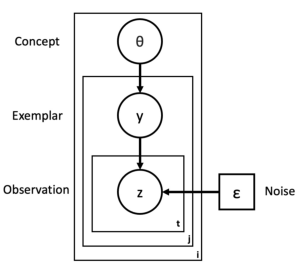
\includegraphics{figs/image-1} 

}

\caption[Graphical representation of our model]{Graphical representation of our model. Circles indicate random variables. The squares indicate fixed model parameters.}\label{fig:image}
\end{figure}
\end{CodeChunk}

Like in our experiment, the learner's task is to decide when to stop
sampling. If they do so rationally, then they should anchor their
sampling behavior to the expected information gain (EIG) of the next
sample. We compute EIG by weighing the information gain from each
possible next observation by the probability of that observation. We
defined information gain as the KL-divergence between the hypothetical
posterior after observing a sample \(z_{t+1}\) and the current
posterior: \begin{eqnarray}
EIG(z_{t+1}) = \sum_{z_{t+1} \in [0,1]} p(z_{t+1}|\theta_t) * KL(\theta_{t+1}, p(\theta_t))
\end{eqnarray} Finally, to get actual sampling behavior from the model,
it has to convert EIG into a binary decision about whether continue
looking at the current sample, or to advance to the next trial. The
model does so using a luce choice between the EIG from the next sample
and a constant EIG from looking away. \begin{eqnarray}
p(look) = \frac{EIG(z_{t+1})}{EIG(z_{t+1})+EIG(world)}
\end{eqnarray} We also studied the behavior of the model when replacing
EIG with other linking hypotheses, such as surprisal (the probability of
a given \(z\) under the \(P(\theta_t)\)) and KL-divergence between the
posterior \(p(\theta_t)\) and the prior \(p(\theta_{t-1})\).

\hypertarget{general-discussion}{%
\section{General Discussion}\label{general-discussion}}

\hypertarget{references}{%
\section{References}\label{references}}

\hypertarget{references-1}{%
\section{References}\label{references-1}}

\setlength{\parindent}{-0.1in} 
\setlength{\leftskip}{0.125in}

\noindent

\bibliographystyle{apacite}


\end{document}
